\begin{name}
	{\tenchude}
	{TOÁN 10}
	{LỚP TOÁN THẦY PHÁT}
	{Thời gian: 90 phút - Không kể thời gian phát đề}
\end{name}
\TN
\Opensolutionfile{ans}[ans/ansDe3-TN1]
\begin{ex}%[0H9N3-1]
	Cho hai điểm $A=\left( 1;2 \right)$ và $B=\left( 5;4 \right)$. Véc-tơ pháp tuyến của đường thẳng $AB$ là
	\choice
	{$\left( -1;-2 \right)$}
	{$\left( 1;2 \right)$}
	{$\left( -2;1 \right)$}
	{\True $\left( -1;2 \right)$}
	\loigiai{
		Ta có $\vec{AB}=\left( 4;\,2 \right)=2\left( 2;\,1 \right)$.\\
		Suy ra véc-tơ pháp tuyến của đường thẳng $AB$ là $\vec{n}_{AB}=\left( -1;\,2 \right)$.
	}
\end{ex}

\begin{ex}%[0H9N3-3]
	Xét vị trí tương đối của hai đường thẳng $d_1\colon x+5=0$ và $d_2\colon y-7=0$.
	\choice
	{Trùng nhau}
	{Song song}
	{\True Vuông góc}
	{Cắt nhau nhưng không vuông góc}
	\loigiai{
		Ta có $d_1\colon x+5=0$ có vectơ pháp tuyến $\overrightarrow{n}_1=\left(1;0 \right)$.\\
		Ta lại có $d_2\colon y-7=0$ có vectơ pháp tuyến $\overrightarrow{n}_2=\left( 0;1 \right)$.\\
		Suy ra $\overrightarrow{n}_1\cdot \overrightarrow{n}_2=1\cdot 0+0\cdot 1=0$.\\
		Vậy $d_1$ và $d_2$ vuông góc nhau.
	}
\end{ex}

\begin{ex}%[0H9N4-1]%[Dự án đề kiểm tra Toán 10 GHKI NH23-24- Lam Nguyen]%[THPT Le Quý Đôn - TPHCM]
	Phương trình nào sau đây \textbf{không} là phương trình đường tròn?
	\choice
	{\True $x^2+y^2-2=0$}
	{$x^2+y^2-y=0$}
	{$x^2+y^2-100y+1=0$}
	{$x^2+y^2-x+y+4=0$}
	\loigiai{
		Phương trình đường tròn có dạng $x^2+y^2-2a x-2by+c=0, (a, b, c \in \mathbb{R})$ với $a^2+b^2>c$. \\
		Dễ thấy $x^2+y^2-2=0$ không phải là phương trình đường tròn.}
\end{ex}

\begin{ex}%[0H9N4-1]%[Dựa án đề kiểm tra Toán khối 10 NH 23 24-Dot15- Đỗ Đường Hiếu]%[THPT Thăng Long - Tp.HCM]
	Xác định tâm $I$ và bán kính $R$ của đường tròn $(C)\colon (x+3)^2+(y-4)^2=49$.
	\choice
	{\True $I(-3;4)$, $R=7$}
	{$I(3;-4)$, $R=7$}
	{$I(3;-4)$, $R=49$}
	{$I(-3;4)$, $R=49$}
	\loigiai{
		Đường tròn $(C)\colon (x+3)^2+(y-4)^2=49$ có tâm $I(-3;4)$, bán kính $R=7$.
	}
\end{ex}

\begin{ex}%[0H9N4-3]%[Dự án đề 4 phần]$%[Tex hóa: Lê Thị Thúy Hằng]
	Trong mặt phẳng với hệ tọa độ $Oxy$, phương trình tiếp tuyến $d$ của đường tròn $(C)\colon (x+2)^2+(y+2)^2=25$ tại điểm $M(2;1)$ là
	\choice
	{$d \colon 3x+4y+14=0$}
	{$d \colon 4x+3y+14=0$}
	{$d \colon 3x+4y-11=0$}
	{\True $d \colon 4x+3y-11=0$}
	\loigiai{
		Ta có tâm của đường tròn có tọa độ $(-2;-2)$.\\
		Phương trình tiếp tuyến của đường tròn tại $M(2;1)\in (C)$ là
		\[(-2-2)(x-2)+(-2-1)(y-1)=0\Leftrightarrow -4x-3y+11=0 \Leftrightarrow 4x+3y-11=0.\]
	}
\end{ex}

\begin{ex}%[0H9N5-2]
	Phương trình nào sau đây là phương chính tắc của một elip?
	\choice
	{$\dfrac{x^2}{4}+\dfrac{y^2}{9}=1$}
	{$\dfrac{x^2}{16}+\dfrac{y^2}{9}=0$}
	{\True $\dfrac{x^2}{25}+\dfrac{y^2}{16}=1$}
	{$\dfrac{x^2}{9}-\dfrac{y^2}{4}=1$}
	\loigiai{
		Phương trình chính tắc của elip có dạng $\dfrac{x^2}{a^2}+\dfrac{y^2}{b^2}=1$, ($a>b$).
	}
\end{ex}

\begin{ex}%[0H9N5-5]%[Duan15-CKII-HN23-24-Trần Xuân Hòa]%[Chuyen Hùng Vương - Phú Thọ]
	Phương trình nào sau đây là phương trình chính tắc của hypebol?
	\choice
	{\True $\dfrac{x^2}{4}-\dfrac{y^2}{9}=1$}
	{$\dfrac{x^2}{9}+\dfrac{y^2}{4}=1$}
	{$\dfrac{x^2}{4}-\dfrac{y^2}{9}=-1$}
	{$\dfrac{x^2}{9}+\dfrac{y^2}{9}=1$}
	\loigiai{
		Phương trình chính tắc của hypebol là $\dfrac{x^2}{4}-\dfrac{y^2}{9}=1$.
	}
\end{ex}

\begin{ex}%[0H9N5-1]
	Cặp điểm nào là các tiêu điểm của elip $(E)\colon \dfrac{x^2}{5}+\dfrac{y^2}{4}=1$?
	\choice
	{\True $F_{1;2}=(\pm1;0)$}
	{$F_{1;2}=(\pm\sqrt{5};0)$}
	{$F_{1;2}=(0;\pm1)$}
	{$F_{1;2}=(0;\pm2)$}
	\loigiai{
		Phương trình tổng quát của elip $(E)\colon\dfrac{x^2}{a^2}+\dfrac{y^2}{b^2}=1 \Rightarrow a=\sqrt{5}$ và $b=2$.\\
		Công thức tiêu điểm của elip là $F_{1;2}=\left(\pm\sqrt{a^2-b^2};0\right)=\left(\pm\sqrt{5-4};0\right)=(\pm1;0)$.
	}
\end{ex}

\begin{ex}%[Dự án EX-10-11-Chuẩn hóa]%[Hoàng Thanh Phương]%[0D3N1-4]
	Điểm nào dưới đây thuộc đồ thị hàm số $y=x^3-x+2$?
	\choice
	{\True $P(1;2)$}
	{$M(1;1)$}
	{$Q(1;3)$}
	{$N(1;0)$}
	\loigiai{ Với $x=1$ ta được $y=1^3-1+2=2$. Vậy điểm $P(1;2)$ thuộc đồ thị hàm số $y=x^3-x+2$.}
\end{ex}

\begin{ex}%[0D3N1-5]
	\immini{Cho hàm số $y=ax^2+bx+c$ có đồ thị $(P)$ như hình vẽ. Khẳng định nào sau đây là đúng?
		\choice
		{Hàm số nghịch biến trên khoảng $(-\infty;4)$ và đồng biến trên khoảng $(4;+\infty)$}
		{Hàm số đồng biến trên khoảng $(-\infty;4)$ và nghịch biến trên khoảng $(4;+\infty)$}
		{\True Hàm số nghịch biến trên khoảng $(-\infty;3)$ và đồng biến trên khoảng $(3;+\infty)$}
		{Hàm số đồng biến trên khoảng $(-\infty;3)$ và nghịch biến trên khoảng $(3;+\infty)$}
	}{
		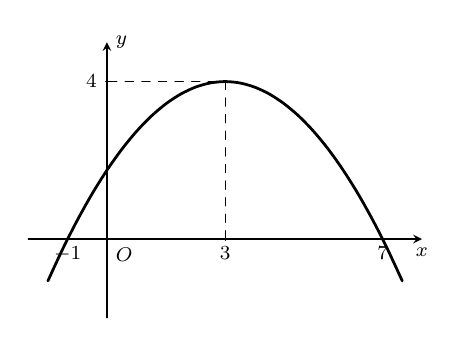
\begin{tikzpicture}[line join=round,line cap=round,>=stealth,scale=0.5,font=\footnotesize]
			\tikzset{every node/.style={scale=0.9}}
			\draw[->] (-2,0)--(8,0) node[below] {$x$};
			\draw[->] (0,-2)--(0,5) node[right] {$y$};
			\draw (0,0) node[below right]{$O$};
			\draw (1pt,4)--(-1pt,4) node [left]{$4$};
			\foreach \i in {-1,3,7}{
					\draw (\i,-1pt)--(\i,1pt) node [below]{$\i$};
				}
			\draw[domain=-1.5:7.5,smooth,line width=1]	plot(\x,{-1/4*(\x)^2+3/2*(\x)+7/4});
			\draw[dashed] (3,0)--(3,4)--(0,4);
		\end{tikzpicture}
	}
	\loigiai{
		Dựa vào đồ thị ta suy ra
		\begin{itemize}
			\item Hàm số đồng biến trên khoảng $(-\infty;3)$.
			\item Hàm số nghịch biến trên khoảng $(3;+\infty)$.
		\end{itemize}
	}
\end{ex}

\begin{ex}%[0D3N2-1]
	Cho parabol $(P)\colon y=3x^2-2x+1$. Điểm nào sau đây là đỉnh của $(P)$?
	\choice
	{$I(0;1)$}
	{\True $I\left(\dfrac{1}{3};\dfrac{2}{3}\right)$}
	{$I\left(-\dfrac{1}{3};\dfrac{2}{3}\right)$}
	{$I\left(\dfrac{1}{3};-\dfrac{2}{3}\right)$}
	\loigiai
	{Ta có $a=3$; $b=-2$; $c=1$ và $\Delta=b^2-4ac=(-2)^2-4\cdot3\cdot 1=-8$.\\
		Tọa độ đỉnh $I\left(-\dfrac{b}{2a};-\dfrac{\Delta}{4a}\right)$ nên $I\left(\dfrac{1}{3};\dfrac{2}{3}\right)$.
	}
\end{ex}

\begin{ex}%[De-chuan-hoa-so-11]%[Đoàn Hùng]%[0D3N2-2]
	Hàm số $y=-2x^2+8x+1$ nghịch biến trên khoảng nào dưới đây?
	\choice
	{$(-\infty;2)$}
	{$(-2;+\infty)$}
	{\True $(2;+\infty)$}
	{$(-\infty;-2)$}
	\loigiai{
		Do $a=-2<0$ nên hàm số đã cho nghịch biến trên khoảng $\left(-\dfrac{b}{a};+\infty\right)$, hay $(2;+\infty)$.
	}
\end{ex}
\Closesolutionfile{ans}

\TNTF
\Opensolutionfile{ans}[ans/ansDe3-TN2]
\begin{ex}%[0H9H3-2]
	Cho đường thẳng $d$ có phương trình $-2x+y-1=0$.
	\choiceTF
	{\True Một vectơ chỉ phương của đường thẳng $d$ là $\overrightarrow u_d =\left(1;2\right)$}
	{\True Phương trình đường thẳng $d'$ đi qua điểm $M(1;3)$ và vuông góc với đường thẳng $d$ là $x+2y-7=0$}
	{\True Khoảng cách từ điểm $N(3;2)$ đến đường thẳng $d$ bằng $\sqrt 5$}
	{Hệ số góc của đường thẳng $d$ là $k=-2$}
	\loigiai{
		\begin{itemchoice}
			\itemch
			Một vectơ chỉ phương của đường thẳng $d$ là $\overrightarrow u_d =\left(1;2\right)$.
			\itemch
			Đường thẳng $d'$ đi qua điểm $M(1;3)$ và vuông góc với đường thẳng $d$ có vectơ pháp tuyến là $\overrightarrow n_{d'}=\left(1;2\right)$ nên có phương trình là $1\cdot (x-1)+2\cdot (y-3)=0 \Leftrightarrow x+2y-7=0$.
			\itemch
			Ta có $\mathrm{d}(N,d)=\dfrac{\left\vert -2\cdot 3+2-1\right\vert}{\sqrt{(-2)^2+1^2}}=\sqrt 5$.
			\itemch
			\begin{align*}
				                & ~ -2x+y-1=0 \\
				\Leftrightarrow & ~y=2x+1.
			\end{align*}
			Hệ số góc của đường thẳng $d$ là $k=2$.
		\end{itemchoice}
	}
\end{ex}

\begin{ex}%[Mức 2]%[Dự án Giảng 10-11 Nhóm Toán & LaTex, Lê Minh Thiện Anh]%[0D3H1-2]
	Cho hàm số $f(x)=x^2$ có đồ thị $(C)$ và hàm số $g(x)=-2x+3$ có đồ thị là đường thẳng $(d)$.
	\choiceTF
	{\True Hàm số $y=\dfrac{\sqrt{g(x)}}{f(x)}$ có tập xác định là $\left(-\infty;\dfrac32\right]\setminus \{0\}$}
	{\True Hàm số $f(x)$ và $g(x)$ cùng đi qua điểm $A(1;1)$}
	{\True Đồ thị $(C)$ nhận trục tung làm trục đối xứng}
	{\True Hàm số $f(|x|)-g(|x|)$ đồng biến trên khoảng $(-1;0)$}
	\loigiai{
		\begin{itemchoice}
			\itemch \textbf{Đúng}.\\
			Hàm số $y=\dfrac{\sqrt{g(x)}}{f(x)}$ xác định khi và chỉ khi
			$$\heva{&f(x)=x^2\neq 0\\&g(x)=-2x+3\geq 0} \Leftrightarrow \heva{& x \ne 0 \\ & x \le \dfrac32}$$
			Vậy hàm số $y=\dfrac{\sqrt{g(x)}}{f(x)}$ có tập xác định là $\left(-\infty;\dfrac32\right]\setminus \{0\}$.
			\itemch \textbf{Đúng}.\\
			Vì $f(1)=1$ và $g(1)=1$ nên hàm số $f(x)$ và $g(x)$ cùng đi qua điểm $A(1;1)$.
			\itemch	\textbf{Đúng}.\\
			Đồ thị hàm số $f(x)=x^2$ nhận trục tung làm trục đối xứng.
			\itemch \textbf{Đúng}.\\
			Ta có $f(|x|)+g(|x|)=|x|^2-2|x|+3=\heva{&x^2-2x+3, \quad x\geq 0\\&x^2+2x+3, \quad x<0}$.\\
			Vì hàm số $y=x^2+2x+3$ đồng biến trên $(-1;+\infty)$ nên cũng đồng biến trên $(-1;0)$.\\
			Vậy hàm số $f(|x|)-g(|x|)$ đồng biến trên khoảng $(-1;0)$.
		\end{itemchoice}
	}
\end{ex}
\Closesolutionfile{ans}

\TNSA
\Opensolutionfile{ans}[ans/ansDe3-TN3]
\begin{ex}%[0H9H4-3]%[tex hóa đề ck2 - form 2025 - đợt 2 - Nguyễn Hữu Thiện]
	Trong mặt phẳng $Oxy$, gọi $d$ là tiếp tuyến của đường tròn $(C): x^2+y^2-4x-2y-20=0$ biết tiếp tuyến $d$ vuông góc với đường thẳng $\Delta: 3x+4y+9=0$ và cắt trục $Ox$ tại điểm có hoành độ dương. Hoành độ giao điểm của $d$ với trục $Ox$ bằng
	\shortans{7,5}
	\loigiai{Đường tròn $(C)$ có tâm $I(2;1)$ và bán kính $R=\sqrt{2^2+1^2+20}=5$.\\
		Đường thẳng $\mathrm{d}$ vuông góc với $\Delta: 3x+4y+9=0 \Rightarrow d: 4x-3y+m=0$.\\
		$d$ là tiếp tuyến của $(C) \Leftrightarrow d(I,d)=R \Leftrightarrow \dfrac{|4\cdot2-3\cdot1+m|}{\sqrt{4^2+(-3)^2}}=5 \Leftrightarrow|m+5|=25.$
		\[
			\Leftrightarrow\hoac{&m+5=25 \\
				&m+5=-25}
			\Leftrightarrow \hoac{&m=20 \\
				&m=-30}
			\Leftrightarrow \hoac{&d: 4x-3y+20=0 \\
				&d: 4x-3y-30=0}.
		\]
		Vì $d$ cắt $Ox$ tại điểm có hoành độ dương nên $d: 4x-3y-30=0$ và toạ độ giao điểm là $(7{,}5;0)$.}
\end{ex}

\begin{ex}%[0H9V3-2]
	Trong mặt phẳng với hệ tọa độ $Oxy$, cho tam giác $ABC$ có trực tâm $H(1;0)$, chân đường cao hạ từ điểm $B$ là điểm $K(0;2)$ và trung điểm cạnh $AB$ là điểm $M(3;1)$. Biết phương trình đường thẳng chứa cạnh $BC$ có dạng $mx+ny+2=0$. Tính $m^2+n^2$.
	\shortans{$25$}
	\loigiai{
		\begin{center}
			\begin{tikzpicture}[line join=round, line cap=round,thick]
				\coordinate (A) at (-1,3);
				\coordinate (B) at (-2,0);
				\coordinate (C) at (3,0);
				\coordinate (M) at ($(A)!0.5!(B)$);
				\coordinate (K) at ($(A)!(B)!(C)$);
				\coordinate (L) at ($(B)!(A)!(C)$);
				\coordinate (H) at (intersection of A--L and B--K);
				\draw(A)--(B)--(C)--cycle (B)--(K) (A)--(L);
				\pic[draw,thin,angle radius=2mm] {right angle = B--K--C};
				\pic[draw,thin,angle radius=2mm] {right angle = A--L--C};
				\foreach \i/\g in {A/90,B/-90,C/-90,M/180,K/45,H/-30}{\draw[fill=black](\i) circle (1.5pt) ($(\i)+(\g:3mm)$) node[scale=1]{$\i$};}
			\end{tikzpicture}
		\end{center}
		Đường cao $BK$ đi qua hai điểm $H$, $K$ nên có phương trình $2x+y-2=0$.\\
		Do $AC \perp B K \Rightarrow AC\colon x-2y+c=0$.\\
		Mà $K \in AC \Rightarrow 0-2.2+c=0 \Rightarrow c=4 \Rightarrow AC\colon x-2y+4=0$.\\
		Giả sữ $A(2a-4;a) \in AC$ và $B(b;2-2b) \in BK$.\\
		Vì $M(3;1)$ là trung điểm của $AB$ nên ta có hệ phương trình:\\
		$\heva{&2a-4+b=2\cdot 3\\
				&a+2-2b=2\cdot 1} \Leftrightarrow
			\heva{&2a+b=10\\
				&a-2b=0} \Leftrightarrow
			\heva{&a=4\\
				&b=2} \Rightarrow A(4;4)$, $B(2;-2)$.\\
		Do đường thẳng chứa cạnh $BC$ đi qua điểm $B$ và nhận vectơ $\overrightarrow{HA}=(3;4)$ làm VTPT nên có phương trình $3x+4y+2=0$.\\
		Vậy $m=3$, $n=4 \Rightarrow m^2+n^2=25$.
	}
\end{ex}

\begin{ex}%[0H9V3-8]
	Trong một khu vực bằng phẳng, ta lấy hai xa lộ vuông góc với nhau làm hai trục tọa độ và mỗi đơn vị độ dài trên trục tương ứng với $1$ km. Cho biết với hệ trục tọa độ vừa chọn thì một trạm viễn thông $T$ có tọa độ $(2;3)$. Một người đang gọi điện thoại di động trên chiếc xe khách chạy trên đoạn cao tốc có dạng một đường thẳng $\Delta$ có phương trình $6x+8y-5=0$. Tính khoảng cách ngắn nhất giữa người đó và trạm viễn thông $T$.
	\shortans{$3{,}1$}
	\loigiai{
		Khoảng cách ngắn nhất giữa người đó và trạm viễn thông $T$ chính là khoảng cách từ $T$ đến đường thẳng $\Delta$. Ta có
		\[ \mathrm{d}(T,\Delta) = \dfrac{|6\cdot2+8\cdot3-5|}{\sqrt{6^2+8^2}} = \dfrac{31}{10} = 3{,}1\text{ km}. \]
	}
\end{ex}

\begin{ex}%[0H9V5-0]
	\immini
	{
		Một công viên có dạng hình elip có độ dài trục lớn bằng $100$ m, độ dài trục bé bằng $80$ m. Người ta muốn trồng hoa trong một hình chữ nhật nội tiếp elip, phần còn lại sẽ trồng cỏ (như hình vẽ). Diện tích trồng hoa lớn nhất bằng bao nhiêu mét vuông?
	}
	{
		\begin{tikzpicture}[line join = round, line cap = round,>=stealth,scale=.8,font=\footnotesize]
			\def\ra{3cm}
			\def\rb{2cm}
			\path
			(0,0) coordinate (A')++(0:2*\ra)coordinate(A)
			($(A')!.5!(A)$)coordinate(O)
			($(O)+(90:\rb)$)coordinate(B)++(-90:2*\rb)coordinate(B')
			($(O)+(50:3cm and 2cm)$) coordinate (M)
			($(O)+(130:3cm and 2cm)$) coordinate (N)
			($(O)+(-130:3cm and 2cm)$) coordinate (P)
			($(O)+(-50:3cm and 2cm)$) coordinate (Q)
			;
			\draw
			(M)--(N)--(P)--(Q)--cycle
			(A')--(A) (B')--(B)
			;
			\fill[pattern=dots,pattern  color=gray]
			(M)--(N)--(P)--(Q)--cycle
			;
			\draw (O) ellipse (3cm and 2cm);
			\foreach \point/\angle in {A'/190,A/-10,B/80,B'/-100}{
					\draw[fill=black](\point)circle(1.2pt)node[shift={(\angle:2.5mm)}]{$\point$};
				}
			\foreach \point in {M,N,P,Q,O}{
					\draw[fill=black](\point)circle(1.2pt);
				}
		\end{tikzpicture}
	}
	\shortans{$4000$}
	\loigiai{
		Phương trình chính tắc của elip $(E)\colon \dfrac{x^2}{a^2}+\dfrac{y^2}{b^2}=1, (a > b > 0)$.\\
		Theo giả thiết ta có $\heva{&
				2a=100\Rightarrow a=50\\&
				2b=80\Rightarrow b=40.}$\\
		Suy ra phương trình elip $(E)\colon \dfrac{x^2}{2500}+\dfrac{y^2}{1600}=1$.\\
		Gọi $M(x_M;y_M)$ là đỉnh hình chữ nhật với $x_M> 0$, $y_M> 0$.\\
		Ta có $\dfrac{x_M^2}{2500}+\dfrac{y_M^2}{1600}=1$.\\
		Diện tích hình chữ nhật là
		\[S=2x_M\cdot 2y_M=4x_My_M=4000\cdot 2\cdot \dfrac{x_M}{50}\cdot \dfrac{y_M}{40}\le 4000\left(\dfrac{x_M^2}{2500}+\dfrac{y_M^2}{1600}\right)=4000\  \mathrm{(m^2)}.\]
	}
\end{ex}
\Closesolutionfile{ans}

\TL
\begin{ex}%[HK1, SoBacNinh, 2023-2024]%[0D3H2-3]
	\,
	\begin{enumerate}
		\item Cho hàm số $y=a{x^2}+bx+2$ có đồ thị là parabol $(P)$. Tìm hàm số đã cho, biết $(P)$ có đỉnh là điểm $I\left(2;6\right)$.
		\item Tìm khoảng đồng biến, nghịch biến của hàm số đã cho và vẽ đồ thị $(P)$ ở câu a.
	\end{enumerate}
	\loigiai{
		\begin{enumerate}
			\item Parabol $y=ax^2+bx+2$ có đỉnh là $I(2;6)$, nên ta có hệ phương trình
			      \[\heva{&-\dfrac{b}{2a}=2\\&y(2)=6}\Leftrightarrow\heva{&4a+b=0\\&4a+2b+2=6}\Leftrightarrow\heva{&a=-1\\&b=4.}\]
			      Vậy hàm số là $y=-x^2+4x+2$.
			\item \,
			      \immini{
				      Hàm số $y=-x^2+4x+2$ có đồ thị là parabol có đỉnh $I(2;6)$ với bề lõm hướng xuống nên hàm số nghịch biến trên $(-\infty;2)$ và đồng biến trên $(2;+\infty)$.
				      Đồ thị hàm số $y=-x^2+4x+2$ là parabol có trục đối xứng $x=2$, đỉnh $I(2;6)$.
				      Bảng giá trị của hàm số $y=-x^2+4x+2$:
				      \begin{center}
					      \begin{tabular}{|c|c|c|c|c|c|c|c|c|c|c|}
						      \hline
						      $x$ & $0$ & $1$ & $2$ & $3$ & $4$ \\
						      \hline
						      $y$ & $2$ & $5$ & $6$ & $5$ & $2$ \\
						      \hline
					      \end{tabular}
				      \end{center}
			      }{
				      \begin{tikzpicture}[scale=.7, font=\footnotesize, line join=round, line cap=round, >=stealth]
					      \draw[->] (-1,0)--(5,0) node[below] {$x$};
					      \draw[->] (0,-1)--(0,7) node[left] {$y$};
					      \draw (0,0) node[below left] {$O$};
					      \draw[domain=-.5:4.5,samples=200] plot (\x,{-1*(\x)^2+4*(\x)+2});
					      \foreach \x in {1,2,3,4}
					      \draw (\x,0) node[below] {$\x$};
					      \foreach \y in {1,2,...,6}
					      \draw (0,\y) node[left] {$\y$};
					      \draw[dashed] (2,-1) node[right]{$x=2$} -- (2,6.5);
				      \end{tikzpicture}
			      }
		\end{enumerate}
	}
\end{ex}

\begin{ex}%[0H9V3-8]
	\immini{
		Để tham gia một phòng tập thể dục, người tập phải trả một khoản phí tham gia ban đầu và phí sử dụng phòng tập. Đường thẳng $\Delta $ ở hình vẽ bên biểu thị tổng chi phí (đơn vị: triệu đồng) để tham gia một phòng thập thể dục theo thời gian tập của một người (đơn vị: tháng).}
	{\begin{tikzpicture}[scale=0.7,>=stealth, font=\footnotesize, line join=round, line cap=round]
			\draw[->] (0,0) node[below left]{$O$}--(8,0) node[below]{tháng};
			\draw[->] (0,0)--(0,6) node[left]{triệu đồng};
			\draw (7,5)node[right]{$A$}--(0,1.5)node[midway,above]{$\Delta$};
			\draw[dashed] (7,0)node[below]{$7$}--(7,5)--(0,5)node[left]{$5$};
			\fill[black] (7,0)circle(1pt) (7,5)circle(1pt) (0,5)circle(1pt) (0,1.5)node[left]{$1{,}5$}circle(1pt) (0,1.5)node[below right]{$B$};
		\end{tikzpicture}
	}
	\noindent
	Tính tổng chi phí mà người đó phải trả khi tham gia phòng tập thể dục với thời gian $12$ tháng.
	\loigiai{
	$\Delta $ qua $A(7;5)$ và $B(0;1{,}5)$, nhận $\overrightarrow{AB}=(-7;-3{,}5)$ làm vectơ chỉ phương có phương trình là $\heva{&=7-7t\\&y=5-3{,}5t}\,(t\in\mathbb{R}$).\\
	Tổng chi phí mà người đó phải trả khi tham gia phòng tập thể dục với thời gian $12$ tháng là
	$x=12$ thay vào phương trình của $\Delta $ ta được
	\[\heva{&12=7-7t\\&y=5-3{,}5t}  \Leftrightarrow \heva{&12=7-7t\\&y=5-3{,}5t}\Leftrightarrow\heva{&t=\dfrac{-5}{7}\\&y=7{,}5.}\]
	Vậy tổng chi phí mà người đó phải trả khi tham gia phòng tập thể dục với thời gian $12$ tháng là $7{,}5$ triệu đồng.
	}
\end{ex}

\begin{ex}%[Nguyễn Cường- BG Toán 10]%[0D2T2-5]
	Một cửa hàng cho thuê sách cũ có quy định: Nếu khách hàng là hội viên của cửa hàng thì phải đóng phí $70000$ đồng/năm và được thuê sách với giá $6000$ đồng/quyển, còn nếu khách hàng không là hội viên phải thuê sách với giá $10000$ đồng/quyển. Gọi $y$ (đồng) là tổng số tiền khách hàng phải trả trong một năm và $x$ là số quyển sách thuê trong một năm.
	\begin{listEX}
		\item Lập hàm số của $y$ theo $x$ với khách hàng là hội viên và với khách hàng không là hội viên của cửa hàng.
		\item Anh Nam là một hội viên của cửa hàng, năm vừa rồi anh Nam trả cho cửa hàng tổng cộng
		$322000$ đồng. Hỏi nếu anh Nam không là hội viên của cửa hàng thì năm vừa rồi anh phải trả
		cho cửa hàng bao nhiêu tiền?
	\end{listEX}
	\loigiai
	{
		\begin{enumerate}
			\item Đối với khách hàng hội viên ta có $y=70000+6000x$.\\
			      Đối với khách hàng không hội viên ta có $y=10000x$.
			\item Thế $y=322000$ vào $y=70000+6000x$, ta có $320000=70000+6000x \Leftrightarrow x=42$.\\
			      Thế $x=42$ vào $y=10000x$, ta có $y=420000$.\\
			      Vậy năm vừa rồi nếu không là hội viên anh Nam phải trả $420000$ đồng.
		\end{enumerate}
	}
\end{ex}


% \HetDe
% \label{De3}
% %
% \cleardoublepage
% \setcounter{page}{1}
% \rfoot{Trang \thepage/\pageref{DA3} - Đáp án trắc nghiệm Mã đề 3}
% \begin{center}
% 	\bfseries ĐÁP ÁN TRẮC NGHIỆM MÃ ĐỀ 3
% \end{center}

% \inputansbox{10}{ans/ansDe3-TN1}
% \inputansbox[3]{2}{ans/ansDe3-TN2}
% \inputansbox{3}{ans/ansDe3-TN3}
% \label{DA3}
%
